\section{Terminologia e concetti}
L'architettura di Von Neumann è composta da quattro componenti principali:
\begin{enumerate}
	\item memoria;
	\item unità di controllo (CU): recupera istruzioni/dati dalla memoria, decodifica le istruzioni e poi in \textbf{sequenza} coordina le operazioni per portare a termine il compito programmato;
	\item unità logico aritmetica (ALU): esegue operazioni aritmetiche di base;
	\item sistemi di I/O (input/output): interfaccia uomo-macchina.
\end{enumerate}
La \textbf{tassonomia classica di Flynn} distingue le architetture di computer multiprocessore in base a come possono essere classificate in due dimensioni indipendenti di \textbf{istruzioni} e \textbf{dati}.
Nella tassonomia di Flynn, vengono identificate cinque componenti:
\begin{enumerate}
	\item IS (Instruction Stream): ovvero il flusso di istruzioni del programma che deve essere eseguito;
	\item DS (Data Stream): il flusso degli operandi e dei risultati dei programmi che sono in esecuzione;
	\item CU (Control Unit): elemento funzionale (chi esegue il fetch e il decode, ovvero il recupero e la decodifica dei dati/istruzioni);
	\item PU (Processing Unit): unità funzionale composta dalla ALU e dai registri. Esegue le istruzioni;
	\item MM(Main Memory): la memoria dove i dati e le istruzioni sono allocati.
\end{enumerate}
Le possibili classificazioni sono:
\begin{enumerate}
	\item SISD (Single Instruction Single Data): la CU recupera le istruzioni dalla MM, mentre la PU esegue le istruzioni interagendo con MM per modificare i dati (figura \ref{fig:sisd});
	\begin{figure}[th]
		\centering
		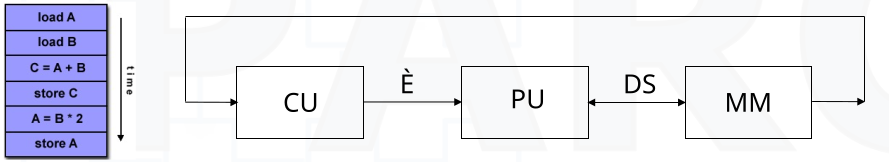
\includegraphics[width=0.7\linewidth]{img/sisd}
		\caption{Single Istruction Single Data.}
		\label{fig:sisd}
	\end{figure}
	\item SIMD (Single Instruction Multiple Data): tutte le unità di elaborazione eseguono la stessa istruzione in ogni dato ciclo di clock; ogni unità di elaborazione può operare su un dato diverso (figura \ref{fig:simd}); è ideale per problemi specializzati caratterizzati da un elevato grado di regolarità, come l'elaborazione grafica o l'elaborazione di immagini; esecuzione sincrona (\textbf{lockstep}) e deterministica
	\begin{figure}[th]
		\centering
		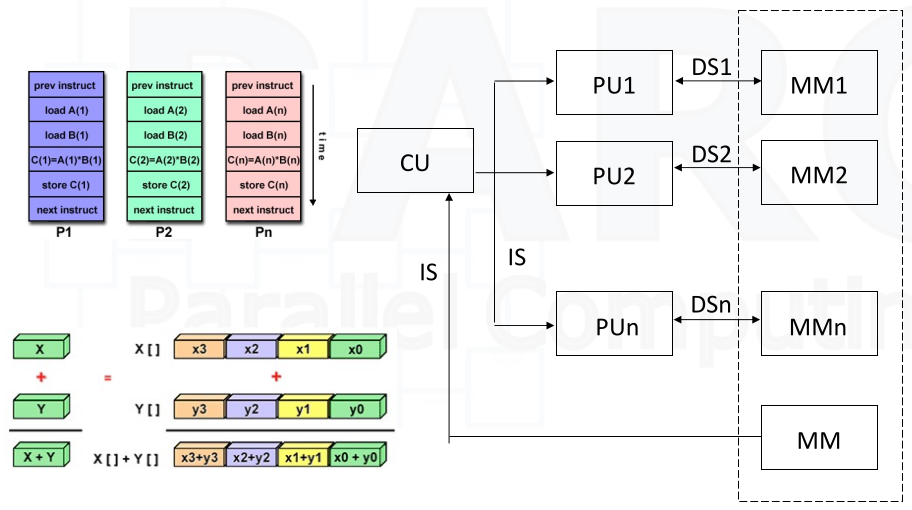
\includegraphics[width=0.7\linewidth]{img/simd}
		\caption{Single Istruction Multiple Data.}
		\label{fig:simd}
	\end{figure}

	\item MISD (Multple Instruction Single Data): un singolo flusso di dati viene immesso in più unità di elaborazione che opera sui dati in modo indipendente tramite flussi di istruzioni indipendenti. Sono esistiti pochi esempi reali di questa classe di computer paralleli (figura \ref{fig:misd});
	\begin{figure}[th]
		\centering
		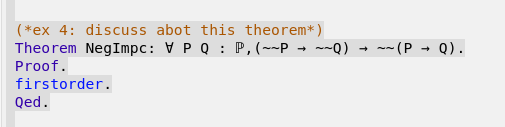
\includegraphics[width=0.7\linewidth]{img/misd}
		\caption{Multiple Instruction Single Data.}
		\label{fig:misd}
	\end{figure}

	\item MIMD (Multple Instruction Multple Data): è il tipo più comune di computer parallelo; ogni processore può eseguire un flusso di istruzioni diverso e lavorare con un flusso di dati diverso. L'esecuzione può essere sincrona o asincrona, deterministica o non deterministica (figura \ref{fig:mimd}).
	\begin{figure}[!th]
		\centering
		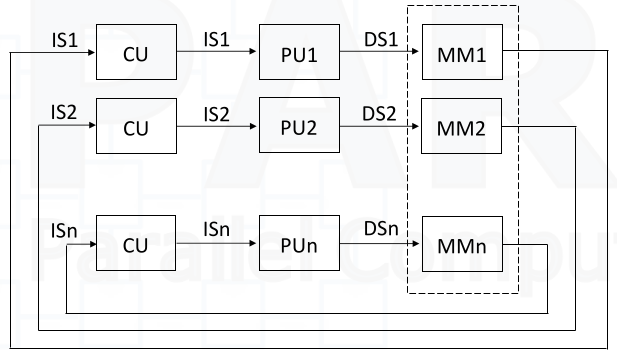
\includegraphics[width=0.7\linewidth]{img/mimd}
		\caption{Multiple Instruction Multiple Data.}
		\label{fig:mimd}
	\end{figure}

\end{enumerate}
\subsection{Terminologia delle architetture parallele}

	\begin{longtable}{|m{0.28\linewidth}|m{0.62\linewidth}|}
		\hline
		\textbf{Termine} & \textbf{Significato}
		\\
		\hline
		\textbf{Task (sequenziale)} & È un'unità di esecuzione o di lavoro di un programma o di un sottoprogramma. Le istruzioni sono eseguite sequenzialmente ovvero non in parallelo.
		\\
		\hline
		\textbf{Task parallelo}& È un task che può essere eseguito in modo sicuro su più processori. Ciascuna istruzione di un task può essere eseguita in maniera concorrente.
		\\
		\hline
		\textbf{Esecuzione seriale} & È l'esecuzione di un programma in sequenza, una dichiarazione alla volta. Nel senso più semplice questo accade su una macchina con un processore. Tuttavia, praticamente tutte le attività parallele avranno sezioni di un programma parallelo che devono essere eseguite in serie.
		\\
		\hline
		\textbf{Esecuzione parallela} & È l'esecuzione di un programma da più di un task, in cui ogni attività è in grado di eseguire la stessa o una diversa istruzione simultaneamente.
		\\
		\hline
		\textbf{Pipelining} & Suddivisione di un compito in passaggi eseguiti da diverse unità di elaborazione, con input che scorrono proprio come una catena di montaggio; un tipo di calcolo parallelo.  La pipeline è un tipo di architettura hardware utilizzata nel progetto dei microprocessori per incrementarne la produttività, ovvero la quantità di istruzioni eseguite nell'unità di tempo. Le istruzioni possono essere di un programma sequenziale. La pipeline può riferirsi anche ad una pipeline di task (ottimizzazione per GPU).
		\\
		\hline
		\textbf{Memoria condivisa} & Dal punto di vista strettamente hardware, descrive un'architettura informatica alla quale tutti i processori hanno accesso diretto (solitamente basato su bus) alla memoria fisica comune; dal punto di vista software, descrive un modello in cui le attività parallele hanno tutte la stessa "immagine" di memoria (\textbf{spazio di indirizzamento comune}) e possono indirizzarsi e accedervi direttamente alle stesse locazioni di memoria logiche indipendentemente da dove esiste effettivamente la memoria fisica. Se lo spazio di indirizzamento non fosse condiviso, si parla di \textbf{memoria distribuita} (che è il contrario della memoria condivisa).
		\\
		\hline
		\textbf{Multiprocessore simmetrico (SMP)} & Architettura hardware in cui più processori condividono un unico spazio di indirizzi e accedono a tutte le risorse; la computazione avviene su memoria condivisa.
		\\
		\hline
		\textbf{Memoria distribuita} & Dal punto di vista hardware, si riferisce all'accesso alla memoria basato sulla rete per la memoria fisica che non è in comune. Il termine può fare riferimento anche ad un'implementazione software dove le attività possono vedere solo la memoria della macchina locale su una vista logica e devono utilizzare comunicazioni per accedere alla memoria su altre macchine su cui sono in esecuzione altre attività.
		\\
		\hline
		\textbf{Comunicazione} & Le attività parallele in genere necessitano di scambiare dati. Esistono tuttavia diversi modi per ottenere questo risultato, ad esempio tramite un bus di memoria condiviso o tramite una rete, tuttavia l'evento effettivo dello scambio di dati viene comunemente definita \emph{comunicazione} indipendentemente dal metodo utilizzato.
		\\
		\hline
		\textbf{Sincronizzazione} & È il coordinamento di attività parallele in tempo reale, molto spesso associato a comunicazioni. Spesso implementate da stabilire un punto di sincronizzazione all'interno di un'applicazione in cui un'attività non può procedere oltre finché un'altra attività non raggiunge lo stesso punto o logicamente equivalente. La sincronizzazione di solito comporta l'attesa di almeno un'altra attività e può quindi causare un aumento del tempo di esecuzione del clock delle applicazioni parallele.
		\\
		\hline
		\textbf{Granularità} & Nel calcolo parallelo, la granularità è una misura quantitativa del rapporto tra il calcolo e la comunicazione. La granularità può essere:
		\begin{itemize}
			\item \textbf{grossolana:} tra gli eventi di comunicazione vengono eseguite quantità di lavoro computazionale relativamente grandi;
			\item \textbf{fine:} tra gli eventi di comunicazione vengono eseguite quantità di lavoro computazionale relativamente piccole.
		\end{itemize}
		\\
		\hline
		\textbf{Accelerazione osservata} & È definita come: $speedup = \frac{execTimeSerial}{execTimeParallel}$ e rappresenta uno degli indicatori più semplici e utilizzati per la performance di un programma parallelo.
		\\
		\hline
		\textbf{Overhead parallelo} & È l'ammontare di tempo richiesto per coordinare task paralleli anziché per eseguire la parte utile del lavoro. L'overhead parallelo può includere fattori come:
		\begin{itemize}
			\item tempo di avvio dei task;
			\item tempo per le sincronizzazioni tra task;
			\item tempo per le comunicazioni di dati tra task;
			\item overhead del software imposto da compilatori paralleli, librerie, strumenti, sistema operativo, \dots
			\item tempo di completamento dei task.
		\end{itemize}
		\\
		\hline
		\textbf{Massivamente parallelo} &  Si riferisce all'hardware che comprende un dato sistema parallelo, dotato di molti processori. Il significato di "molti" continua ad aumentare, ma attualmente i computer più grandi possono essere costituiti da processori che si contano nell'ordine di centinaia di migliaia.
		\\
		\hline
		\textbf{Imbarazzantemente parallelo} & Indica l'azione di risolvere simultaneamente task simili ma indipendenti; la coordinazione tra task è quasi assente o completamente assente.
		\\
		\hline
		\textbf{Scalabilità} & Si riferisce alla capacità di un sistema parallelo (HW e/o SW) di dimostrare un aumento proporzionale della velocità parallela con l'aggiunta di più processori. I fattori che contribuiscono alla scalabilità includono:
		\begin{itemize}
			\item HW: in particolare larghezze di banda della memoria-cpu e comunicazioni attraverso la rete;
			\item l'algoritmo dell'applicazione;
			\item relativo all'overhead parallelo;
			\item caratteristiche specifiche dell'applicazione e codifica
		\end{itemize}
		\\
		\hline
		\textbf{Processori multi-core} & Processori in cui sono presenti più core su un singolo chip
		\\
		\hline
		\textbf{Computazione in cluster} & Utilizzo di una combinazione di unità di calcolo di base (processori, reti o SMP) per costruire un sistema parallelo.
		\\
		\hline
		\textbf{Supercomputing / Calcolo ad alte prestazioni} & Utilizzo delle macchine più veloci e più grandi al mondo per risolvere problemi molto complessi (le unità di calcolo di cui sono composti non devono necessariamente essere omogenei).
		\\
		\hline
		\textbf{Edge computing} & Distribuire il paradigma informatico che avvicina il calcolo e l'archiviazione dei dati al luogo in cui si trovano. Necessario per migliorare i tempi di risposta e risparmiare larghezza di banda.
		\\
		\hline
	\end{longtable}
\subsubsection{Tipi di memoria}
La \textbf{cache} è un'area di memoria estremamente veloce ma solitamente di un basso ordine di grandezza di capacità. Il suo scopo è di velocizzare l'esecuzione dei programmi.

La figura \ref{fig:uma} è un esempio di memoria condivisa. I computer paralleli con memoria condivisa variano ampiamente, ma generalmente hanno in comune la capacità di tutti i processori di accedere a tutta la memoria come spazio di indirizzi globale. Più processori possono funzionare in modo indipendente ma condividono le stesse risorse di memoria. Le modifiche in una posizione di memoria effettuate da un processore sono visibili a tutti gli altri processori. Le macchine a memoria condivisa possono essere divise in due classi principali in base ai tempi di accesso alla memoria:
\begin{enumerate}
	\item UMA (Unified Memory Access): i processori sono identici, il tempo e la modalità di accesso alla memoria sono gli stessi per tutti i processori (figura \ref{fig:uma}). A volte chiamato \textbf{CC-UMA} (\emph{Cache Coherent UMA}). \textbf{Coerenza} della cache significa che se un processore aggiorna una posizione nella memoria condivisa, tutti gli altri processori vengono a conoscenza dell'aggiornamento. La coerenza della cache viene raggiunta a livello hardware.
	\begin{figure}[th]
		\centering
		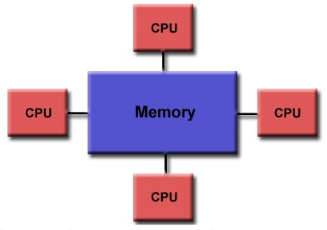
\includegraphics[width=0.7\linewidth]{img/UMA}
		\caption{Memoria condivisa di classe UMA.}
		\label{fig:uma}
	\end{figure}
	\item NUMA (Not Unified Memory Access): spesso realizzato collegando fisicamente due o più SMP; un SMP può accedere direttamente alla memoria di un altro SMP. Non tutti i processori hanno lo stesso tempo di accesso a tutte le memorie. L'accesso alla memoria attraverso il bus è più lento. Se viene mantenuta la coerenza della cache, la memoria si dice \textbf{CC-NUMA} (\emph{Cache Coherent NUMA}).
	\begin{figure}[th]
		\centering
		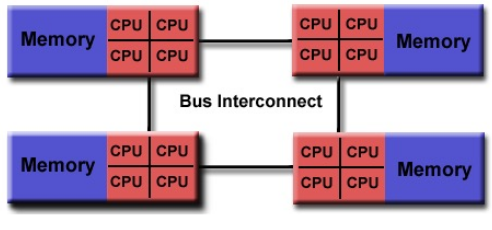
\includegraphics[width=0.7\linewidth]{img/NUMA}
		\caption{Memoria condivisa di classe NUMA.}
		\label{fig:numa}
	\end{figure}
\end{enumerate}
	\subsubsection{Vantaggi e svantaggi di una memoria condivisa.} Vantaggi di avere una memoria condivisa sono:
	\begin{itemize}
		\item lo spazio degli indirizzi globale fornisce alla memoria una prospettiva di programmazione user-friendly; \item la condivisione dei dati tra le attività è veloce e uniforme alla vicinanza della memoria alle CPU.
	\end{itemize}
	Gli svantaggi sono:
	\begin{itemize}
		\item mancanza di scalabilità tra memoria e CPU; \item diventa sempre più difficile e costoso progettare e produrre macchine a memoria condivisa con un numero sempre crescente di processori.
	\end{itemize}

Come i sistemi di memoria condivisa, i sistemi di memoria distribuita variano ampiamente ma condividono una caratteristica comune. Per connettere la memoria inter-processore, il sistema richiede una rete di comunicazione.
I processori hanno la propria memoria locale. Gli indirizzi di memoria in un processore non vengono mappati su un altro processore, quindi non esiste il concetto di \textbf{spazio degli indirizi globale} su tutti i processori.

Poiché ogni processore ha la propria memoria locale, funziona in modo indipendente. Le modifiche apportate alla memoria non hanno effetto sulla memoria degli altri processori. Pertanto, il concetto di coerenza della cache non si applica.
Quando un processore ha bisogno di accedere ai dati in un altro processore, solitamente è compito del programmatore definire esplicitamente come e quando i dati vengono comunicati. Anche la sincronizzazione tra i compiti è responsabilità del programmatore.

\subsubsection{Vantaggi e svantaggi di una memoria distribuita.} I vantaggi di avere una memoria distribuita sono:
\begin{itemize}
	\item la \textbf{memoria} è \textbf{scalabile} con il numero di processori; \item aumenta il numero di processori e la dimensione della memoria aumenta proporzionalmente; \item ogni processore può accedere rapidamente alla propria memoria senza interferenze e senza il sovraccarico sostenuto nel tentativo di mantenere la coerenza della cache. \item in termini di costi, la memoria distribuita è efficace, poiché può utilizzare processori e reti standard disponibili in commercio.
\end{itemize}
Gli svantaggi sono i seguenti:
\begin{itemize}
	\item il programmatore è responsabile per molti dei dettagli associati alla comunicazione dei dati tra i processori. \item potrebbe essere difficile mappare su questa organizzazione della memoria le strutture dati esistenti, basate sulla memoria globale; \item tempi di accesso alla memoria non uniforme (NUMA).
\end{itemize}
\subsubsection{Memoria ibrida distribuita-condivisa} I computer più grandi e veloci del  mondo oggi impiegano questo tipo di architettura (figura \ref{fig:hybrid-memory}). Il componente di memoria condivisa è solitamente una macchina SMP coerente con la cache. I processori su un dato SMP possono indirizzare la memoria di quella macchina come globale.

\begin{figure}[th]
	\centering
	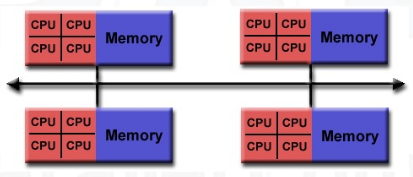
\includegraphics[width=0.7\linewidth]{img/hybrid-memory}
	\caption{Memoria ibrida distribuita-condivisa.}
	\label{fig:hybrid-memory}
\end{figure}

Il componente di memoria distribuita è il collegamento in rete di più SMP. Gli SMP conoscono solo la propria memoria, non quella di un altro SMP. Pertanto, le comunicazioni di rete sono necessarie per spostare i dati da un SMP all'altro. I vantaggi e gli svantaggi sono tutto ciò che è comune alle architetture di memoria e distribuita.
